\subsection{Canal com apagamento 2}

\begin{questions}
\question{
Considere o canal discreto sem memória 
representado na figura abaixo.
\begin{figure}
\centering
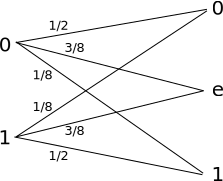
\includegraphics[width=0.3\linewidth]{../images/canale.pdf}
\end{figure}

\begin{parts}
\part Qual é a capacidade do canal?

\part Qual é a distribuição de $X$ que alcança a capacidade do canal? ($p = (p_0, p_1)$)

\end{parts}
}

\begin{solution}

A capacidade de canal é dada por
\begin{align}
C &= \max_{p(x)} I(X;Y) \nonumber \\
  &= \max_{p(x)} H(Y) - H(Y|X) \nonumber \\
  &= \max_{p(x)} H(Y) - H\left( \frac{1}{2}, \frac{3}{8}, \frac{1}{8} \right) \nonumber \\
  &= H\left( \frac{5}{16}, \frac{6}{16}, \frac{5}{16} \right) - H\left( \frac{1}{2}, \frac{3}{8}, \frac{1}{8} \right) \nonumber \\
  &= \frac{5}{16} (4 - \log 5) + \frac{3}{8} (3 - \log 3) + \frac{5}{16} (4 - \log 5) - \frac{1}{2} - \frac{3}{8} (3 - \log 3) - \frac{3}{8} \nonumber \\
  &= \frac{13}{8} - \frac{5}{8} \log 5 .
\end{align}
Utilizamos a simetria para identificar que a distribuição $p(x)$ que maximiza a $H(Y)$ é $\left( \frac{1}{2}, \frac{1}{2} \right)$,
levando à distribuição $\left( \frac{5}{16}, \frac{6}{16}, \frac{5}{16} \right) $ na saída.


\end{solution}
\end{questions}
